\documentclass[letterpaper, 11pt]{article}

\usepackage{lastpage, url, marginnote, siunitx, circuitikz, kantlipsum, graphicx}

\usepackage[margin=1in]{geometry}
%\geometry{hscale=.6, vscale=.8, hmarginratio=2:1, vmarginratio=1:1, marginparwidth=.18\paperwidth, ignoremp}
%\geometry{marginparwidth=.1\paperwidth}

%\usepackage[T1]{fontenc}

%\usepackage[explicit]{titlesec}
%\titlespacing*{\section}{\dimexpr -\marginparsep-\marginparwidth}{*4}{*1}
%\titleformat{\section}[runin]{\large\bfseries\titlerule[.5pt]\filright}{\makebox[1em][c]{\thesection}}{1em}{\parbox[t]{\dimexpr\marginparwidth-2em}{#1}\hskip\marginparsep\mbox{}}[\newline]

%\titlespacing*{\subsection}{\dimexpr -\marginparsep-\marginparwidth}{*4}{*1}
%\titleformat{\subsection}[runin]{\large\bfseries\titlerule[.5pt]\filright}{\makebox[1em][c]{\thesection}}{1em}{\parbox[t]{\dimexpr\marginparwidth-2em}{#1}\hskip\marginparsep\mbox{}}[\newline]

\usepackage{enumitem}
\newlist{steps}{enumerate}{1}
\setlist[steps]{label=Step \arabic*, font=\bfseries, leftmargin=-\marginparsep, itemindent=\marginparsep, align=right}

\usepackage{fancyhdr}
\pagestyle{fancy}
\fancyhf{}
\fancyhfoffset[lh,lf]{\dimexpr\marginparwidth+\marginparsep}
\fancyhf[lh]{UCD EEC 134}
\fancyhf[ch]{}
\fancyhf[rh]{}
%\fancyhf[lf]{left foot}
%\fancyhf[cf]{centre foot}
\fancyhf[rf]{Page \thepage /\pageref{LastPage}}
%\renewcommand{\footrulewidth}{.4pt}

%%%%%%%%%%%%%%%
%%%% Tikz definitions
%%%%%%%%%%%%%%%
%\tikzstyle{Uno}=[rectangle,fill=white,draw,line width=0.5mm]

\begin{document}

\title{Appendix A: Teensy Primer}
\author{Xiaoguang ``Leo'' Liu\\lxgliu@ucdavis.edu}
\date{Last updated: \today}

\maketitle

\section{Introduction}
The Teensy is a Cortex-M4 based microcontroller development platform in a very small footprint. All the programming and data connection are done through the USB port, using a standard ``Mini-B'' USB adapter. 

The Teensy 3.1 features a very capable MK20DX256 32-bit Cortex-M4 processor running at a clock speed of 72 MHz. The processing units has 256K flash memory, 64K RAM, and 2K EEPROM. The peripherals include 21 analog input, 12 PWM output, 3 UART channels, 2 I2C channels, and 1 SPI channel. Worth noting is that the analog and digital pins are compatible with 5-V signals. 

%\begin{figure}
%	\centering
%	\includegraphics{lab1_system}
%	\caption{}
%	\label{fig:lab1_system}
%\end{figure}
[include pin mapping]

The input and output pins of the Teensy are arranged in two parallel rows with a spacing that is compatible with most breadboards. This makes it quite easy to prototype a project when more electronic components are needed.

\begin{figure}[ht]
	\centering
	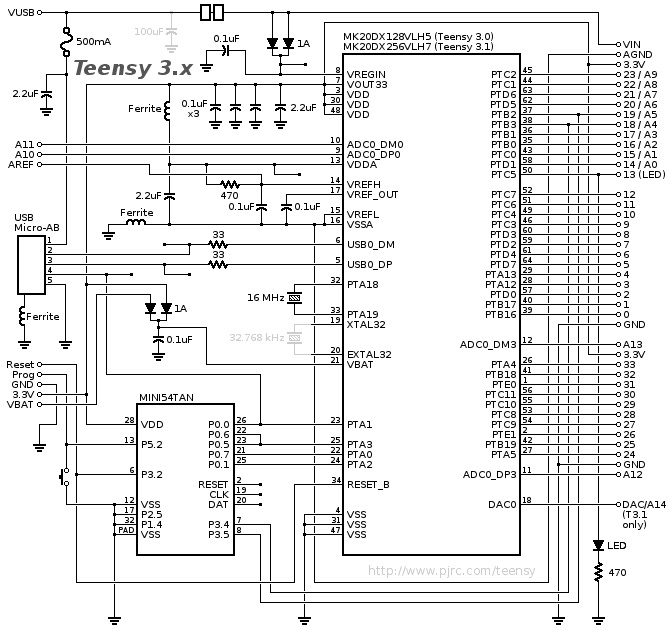
\includegraphics[width=4.5in]{teensy_sch.png}
	\caption{Schematic of the Teensy 3.0/3.1 development platform~\cite{bib:teensy_sch}.}
	\label{fig:teensy_sch}
\end{figure}

\begin{figure}[ht]
	\centering
	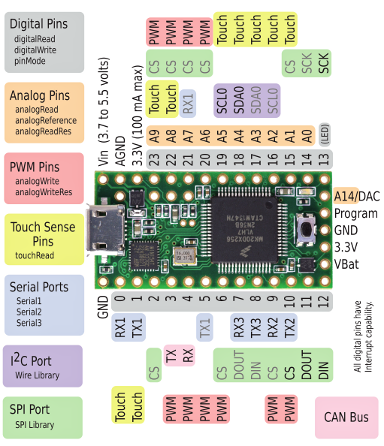
\includegraphics[width=3.5in]{teensy_pinout.png}
	\caption{Pinout diagram for the Teensy 3.1~\cite{bib:teensy_pinout}.}
	\label{fig:teensy_pinout}
\end{figure}

\section{Microcontroller basics}

\section{Light up an LED}
Blinking a Light Emitting Diode (LED) is a canonical example in the embedded system world that shares a same popularity as the ``Hello World!'' does in computer programming. There are many ways to turn an LED on and off. The simplest among them is to use a digital output pin to apply the necessary voltage across the LED\footnote{An LED is basically a diode that can emit light when forward biased (anode at a higher electric potential than cathode). The colors of the emitted light of an LED depends on the material composition and the structure of the diode design. The forward voltage drop will also be different for LEDs with different colors.}. 

On the Teensy 3.1, a ``digital high'' is equivalent to roughly 5\,V. Because of the exponential I-V characteristics of the diode, such a large voltage drop across the LED will induce a lot of current, in fact much more than the output circuits in Teensy can handle. Usually a resistor is added to the circuit to prevent this from happening. Similar to a lot of popular microcontroller development platforms, the Teensy has already included an LED with a suitable resistor. If you look at Fig.~\ref{fig:teensy_sch} closely, you will see that an LED and a \SI{470}{\ohm} resistor are connected to pin 13 which is unequivocally labeled as ``LED''. 

So to implement our blinking LED example, we don't actually need to build any circuit. All we need to do is to load up the proper program, compile, and download to the Teensy. The program reads as follows: 


\section{Reading digital input}

\section{Using PWM for analog output}

\section{Using interrupts}

\section{Using the timer}

\section{Using the digital to analog converter (DAC)}

\section{Using the memory}

\section{Using the analog to digital converter (ADC)}

\section{Using the audio library}


\begin{thebibliography}{9}

\bibitem{bib:teensy_sch}
  PJRC.com, LLC,
  \emph{Teensy reference: schematic},
	online: \url{https://www.pjrc.com/teensy/schematic.html}, accessed Jun.~23, 2015.

\bibitem{bib:teensy_sch}
  PJRC.com, LLC,
  \emph{Teensy: pinouts},
	online: \url{https://www.pjrc.com/teensy/teensy31.html}, accessed Jun.~23, 2015.
  
\end{thebibliography}

\end{document}